\documentclass[amsmath, amssymb, aip, jmp, reprint]{revtex4-2}
\usepackage{tikz}
\usetikzlibrary{shapes.geometric}
\usetikzlibrary{decorations.markings}

\begin{document}

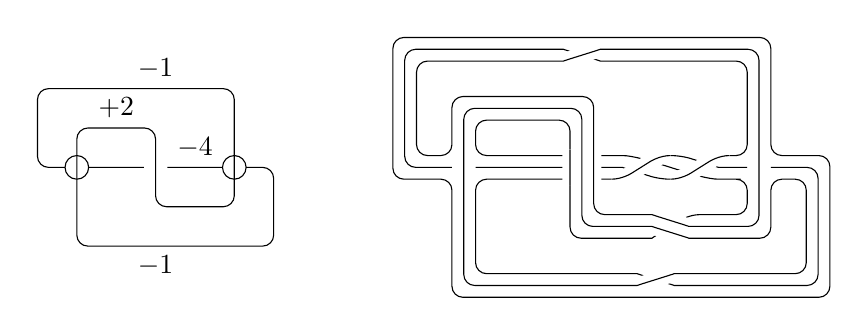
\begin{tikzpicture}
\matrix[column sep = 1.5 cm, row sep = 0.5 cm]{

	% Original graph

	\draw (-1, 0) circle (0.15);
	\draw (1, 0) circle (0.15);
	
	\draw [rounded corners] (-0.15, 0) -- (-0.85, 0) (-1.15, 0) -- (-1.5, 0) -- (-1.5, 1) -- node [above, pos = 0.6] {$-1$} (1, 1) -- (1, -0.5)
		-- (0, -0.5) -- (0, 0.5) -- node [above] {$+2$} (-1, 0.5) -- (-1, -1) -- node [below, pos = 0.4] {$-1$} (1.5, -1) -- (1.5, 0) -- (1.15, 0)
		(0.85, 0) -- node [above] {$-4$} (0.15, 0);

&
	
	% 3-line graph
	
	\begin{scope}[scale = 0.75]
	
	\draw [rounded corners]
		(2, -0.8) cos (1.5, -1) sin (1, -1.2) -- (-0.2, -1.2) -- (-0.2, -0.3) (-0.2, 0.3) -- (-0.2, 0.8) -- (-1.8, 0.8) -- (-1.8, 0.2)
			-- (0.5, 0.2) cos (1.5, 0) sin (2.5, -0.2) -- (2.8, -0.2) -- (2.8, -0.8) -- (2, -0.8)
		(-2.2, 0) -- (-3, 0) -- (-3, 2) -- (-0.5, 2) cos (0, 1.9) sin (0.5, 1.8) -- (2.8, 1.8) -- (2.8, 0.2) -- (2.5, 0.2)
		(1.5, 0.2) cos (2, 0.1) sin (2.5, 0) -- (2.8, 0) (-1.8, 0) -- (0.5, 0) cos (1, -0.1) sin (1.5, -0.2)	 
		(1.5, -2.2) -- (4.2, -2.2) -- (4.2, 0.2) -- (3.2, 0.2) -- (3.2, 2.2) -- (-3.2, 2.2) -- (-3.2, -0.2) -- (-2.2, -0.2) -- (-2.2, -2.2) -- cycle % 0(23) 1(10)
		(0.5, -0.2) -- (-1.8, -0.2) -- (-1.8, -1.8) -- (0.75, -1.8) cos (1.25, -1.9) sin (1.75, -2) -- (4, -2) -- (4, 0)
			-- (3.2, 0) % 0(12), 1(20)
		;
	
	\draw [rounded corners, draw = white, double = black, double distance between line centers = 3 pt, line width = 2.6 pt]
		(0, 0.3) -- (0, 1) -- (-2, 1) -- (-2, -2) -- (0.75, -2) cos (1.25, -1.9) sin (1.75, -1.8) -- (3.8, -1.8)
		-- (3.8, -0.2) -- (3.2, -0.2) -- (3.2, -1.2) -- (2, -1.2) cos (1.5, -1.1) sin (1, -1) -- (0, -1) -- cycle			% 0(13), 1(21)
		(0.2, 0.3) -- (0.2, 1.2) -- (-2.2, 1.2) -- (-2.2, 0.2) -- (-2.8, 0.2) -- (-2.8, 1.8) -- (-0.5, 1.8) cos (0, 1.9) sin (0.5, 2) -- (3, 2)
		-- (3, -1) -- (2, -1) cos (1.5, -0.9) sin (1, -0.8) -- (0.2, -0.8) -- cycle % 0(03), 1(13)
		(-0.2, -0.3) -- (-0.2, 0.3)
		
		(0.5, -0.2) cos (1, 0) sin (1.5, 0.2)
		(1.5, -0.2) cos (2, 0) sin (2.5, 0.2)
		;
		
	\end{scope}

\\
};
\end{tikzpicture}

\end{document}